\section{Appendix}

XXX.  APPENDIX.

\michael{I put this here for now as a placeholder.  Where to put it.  Maybe in a discussion/conclusion if there is space.}

\paragraph{XXX.}
XXX.  THIS VERIFICATION IS NOT ABOUT CONV LAYERS, IT IS ABOUT PL MORE GENERALLY, CORRECT?  WE SHOULD CLARIFY AND SQUISH.
To verify that our approach is meaningful, we need to confirm that the ESD is neither due to a random matrix, nor due to unsually large matrix elements, but, in fact, captures correlations learned from the data. 
We examine typical layer for the pretained AlexNet model (distributed with pyTorch). 
Figure~\ref{fig:alexnet1} displays the ESD for the first slice (or matrix $\mathbf{W}$) of the third Conv2D layer, extracted from a 4-index Tensor of shape $(384, 192, 3, 3)$.  The red line displays the best fit to a random matrix, using the Marchenko pastur theory~\cite{MM}.  We can see the random matrix model does not describe the ESD very well. For comparison, Figure \ref{fig:alexnet2} shows the ESD of the same matrix, randomly shuffled; here looks similar to the red line plot of the orginal ESD.  In fact, the empircal ESD is better modeled with a truncated power law distribtion.
\michael{We may want to give a one-sentence summary of this par and fig at the end of the previous par.}
\charles{Here, on the RMT MP stuff, I think it makes sense to point back}

\begin{figure}[H]
   \centering
   \subfigure[Actual ESD]{
     %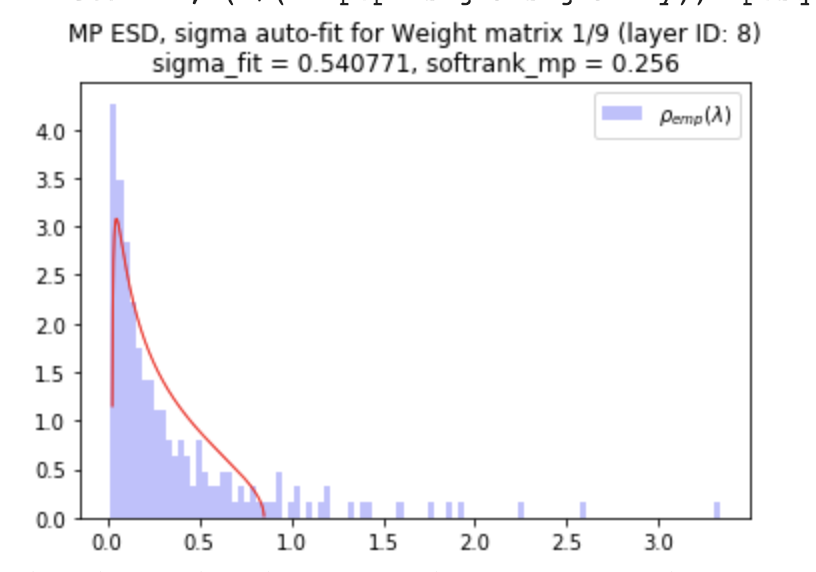
\includegraphics[scale=0.5]{img/alexnet1.png} 
     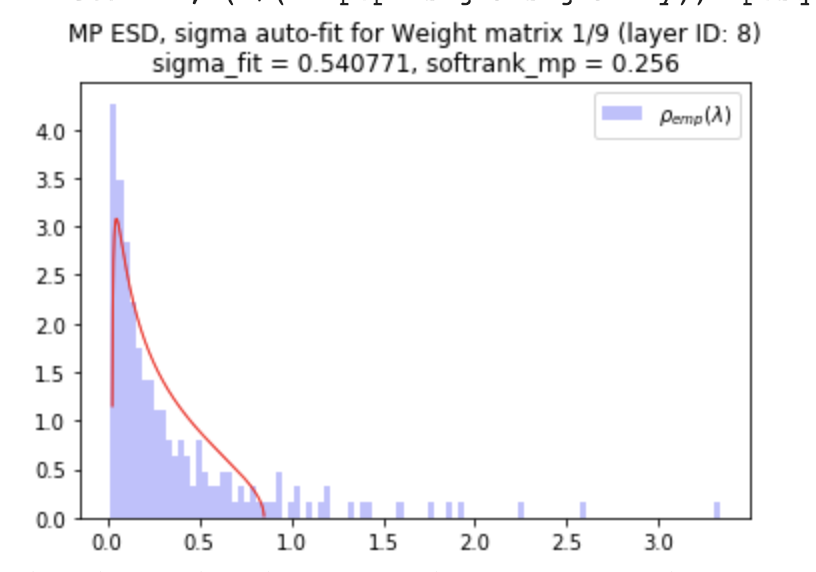
\includegraphics[scale=0.25]{img/alexnet1.png} 
     \label{fig:alexnet1}
   }
   \subfigure[ESD of randomly shuffled matrix]{
      %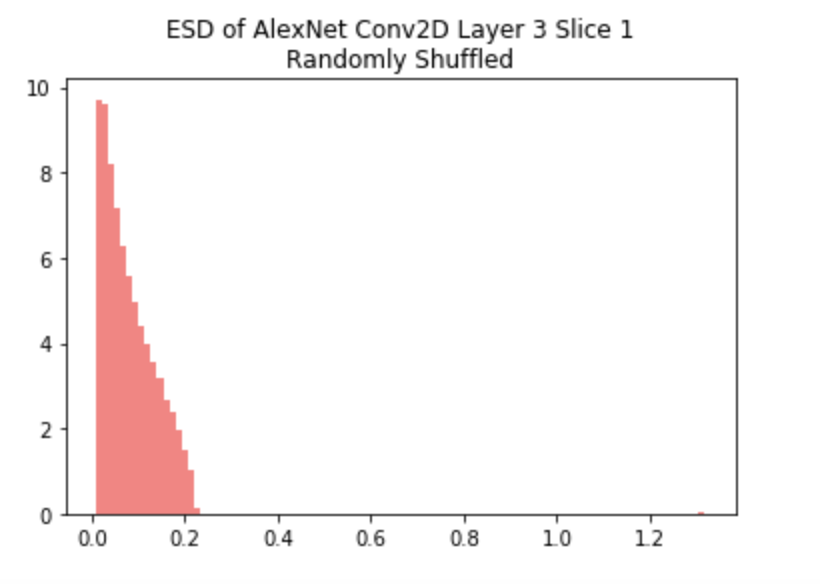
\includegraphics[scale=0.5]{img/alexnet2.png}
      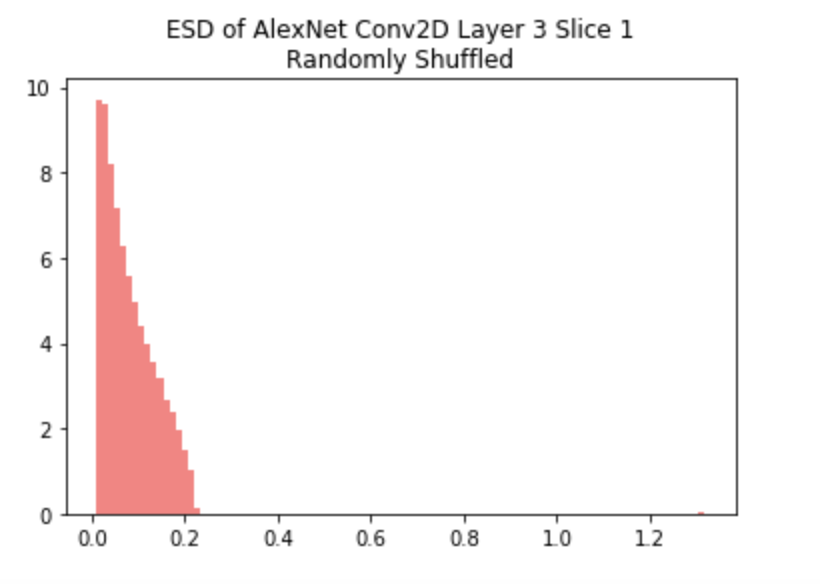
\includegraphics[scale=0.25]{img/alexnet2.png}
      \label{fig:alexnet2}
   }
   \caption{ESD of AlexNet Conv2D pre-Activation map for Layer 3 Slice 1, actual and randomized.
            \michael{Need better figs here.}
           }
   \label{fig:alexnet}
\end{figure}


Although the ESD is \emph{Heavy Tailed}, this does not imply that the orginal matrix $\mathbf{W}$ is itself heavy tailed--only the correlation matrix $\mathbf{X}$ is. 
If $\mathbf{W}$ was, then it would contain 1 or more unusually large matrix elements, and they would dominate the ESD.  
Of course the randomized $\mathbf{W}$ would also be heavy tailed, but its ESD neither resembles the original nor is it heavy tailed. 
So we can rule out $\mathbf{W}$ being heavy tailed.
\michael{These comments seem out of place, since they hold more generally than for the Conv2D layers.}
\charles{Agreed. We could move this up.  We have never really talked about this, but it is essential to explain the difference between assuming W is heavy tailed , which confuses everyone}

These plots tell us that the pre-activation maps of the Conv2D contains significant correlations learned from the data.  
By modeling the ESD with a power law distribution $\lambda^{\alpha}$, we can characterize the amount of correlation learned;
the smaller the exponent $\alpha$, the more correlation in the weight matrix. 
\michael{These comments seem out of place, since they hold more generally than for the Conv2D layers.}

